%%%%%%%%%%%%%%%%%%%%%%%%%%%%%%%%%%%%%%%%%%%%%%%%%%%%%%%%%%%%%%%%%%%%%%%
%%%%  Load the document class and packages                         %%%%
%%%%%%%%%%%%%%%%%%%%%%%%%%%%%%%%%%%%%%%%%%%%%%%%%%%%%%%%%%%%%%%%%%%%%%%
\documentclass[11pt]{report} %LOAD THE DOCUMENT CLASS
%\documentclass[a4paper]{report}
%\usepackage{epsfig}            % to insert PostScript figures

\usepackage{graphicx}
\include{srctex}               % For Latex inverse searc
\usepackage[bf,footnotesize]{caption} % make captions small and label bold

\usepackage[letterpaper,margin=3cm,tmargin=2.75cm,bmargin=3cm]{geometry} 

%%%%%%%%%%%%%%%%%%%%%%%%%%%%%%%%%%%%%%%%%%%%%%%%%%%%%%%%%%%%%%%%%%%%%%%
%%%%  Setup a default path to search for graphics                  %%%%
%%%%%%%%%%%%%%%%%%%%%%%%%%%%%%%%%%%%%%%%%%%%%%%%%%%%%%%%%%%%%%%%%%%%%%%
\graphicspath{
              {images/}
}



\setcounter{secnumdepth}{-1} 
\begin{document}

\section{Introduction}
These are the instructions for building the OpenStage microscope stage controller based around a Rev 2 PCB. The Rev2 board is a prototype and contains some mistakes that you will have to work around. None of these mistakes are show-stoppers, they just result in some cosmetic kludges. \textbf{Read the whole way through this guide before you start soldering.} Think before you solder: you are the first (or one of the first) to build this thing so there may be mistakes in the guide. Please report your experience and any errors you find. Some steps have various solutions: choose the one that works best for you. The Rev 2 board has the following issues, all of which have solutions\footnote{Your board will likely come with the power switch holes drilled out and a serial port connector correctly wired}:

\vspace{2em}

\begin{tabular}{|p{5.5cm}| p{9cm}|}
\hline
Issue & Solution \\
\hline
\hline
LCD header is inverted & Connect LCD to PCB via a ribbon cable, to flip the lines left/right \\
\hline
Serial comms socket is inverted & snip off socket pins 1 and 4. Solder socket into place. Connect solder pads at positions 1 and 5 and also at positions 2 and 4. \\
\hline
Power switch drill holes too small & Drill out (carefully!)\\
\hline
Top left LCD spacer drill hole too close to jumper & Either don't use this spacer or short jumper using solder or wire, this will provide enough room to screw in a spacer. \\
\hline
Some drill holes for case mounting overlap with mounted components & User other drill holes--there are loads. \\
\hline
Motor serial connectors are a little closer to each other & Serial sockets that plug into the connectors do fit side by side (just!)\\
\hline
Connections from Quadstepper motor outputs to Openstage PCB are a bit crap. & 
I'm looking for suggestions! \\
\hline
\end{tabular}

\clearpage

Figure~\ref{frontback} shows the bare PCB, as it looks like before you start. Figure~\ref{finished_1} shows roughly what the board will look like when it's finished, with the components installed. Optional buttons near the top of the front of the board haven't been installed here. The LCD display will \textit{not} just slot into the header, unfortunately, as the connections are backwards. You should probably solder the wiring for the LCD display right at the end. 

\begin{figure}[!ht]
\centering
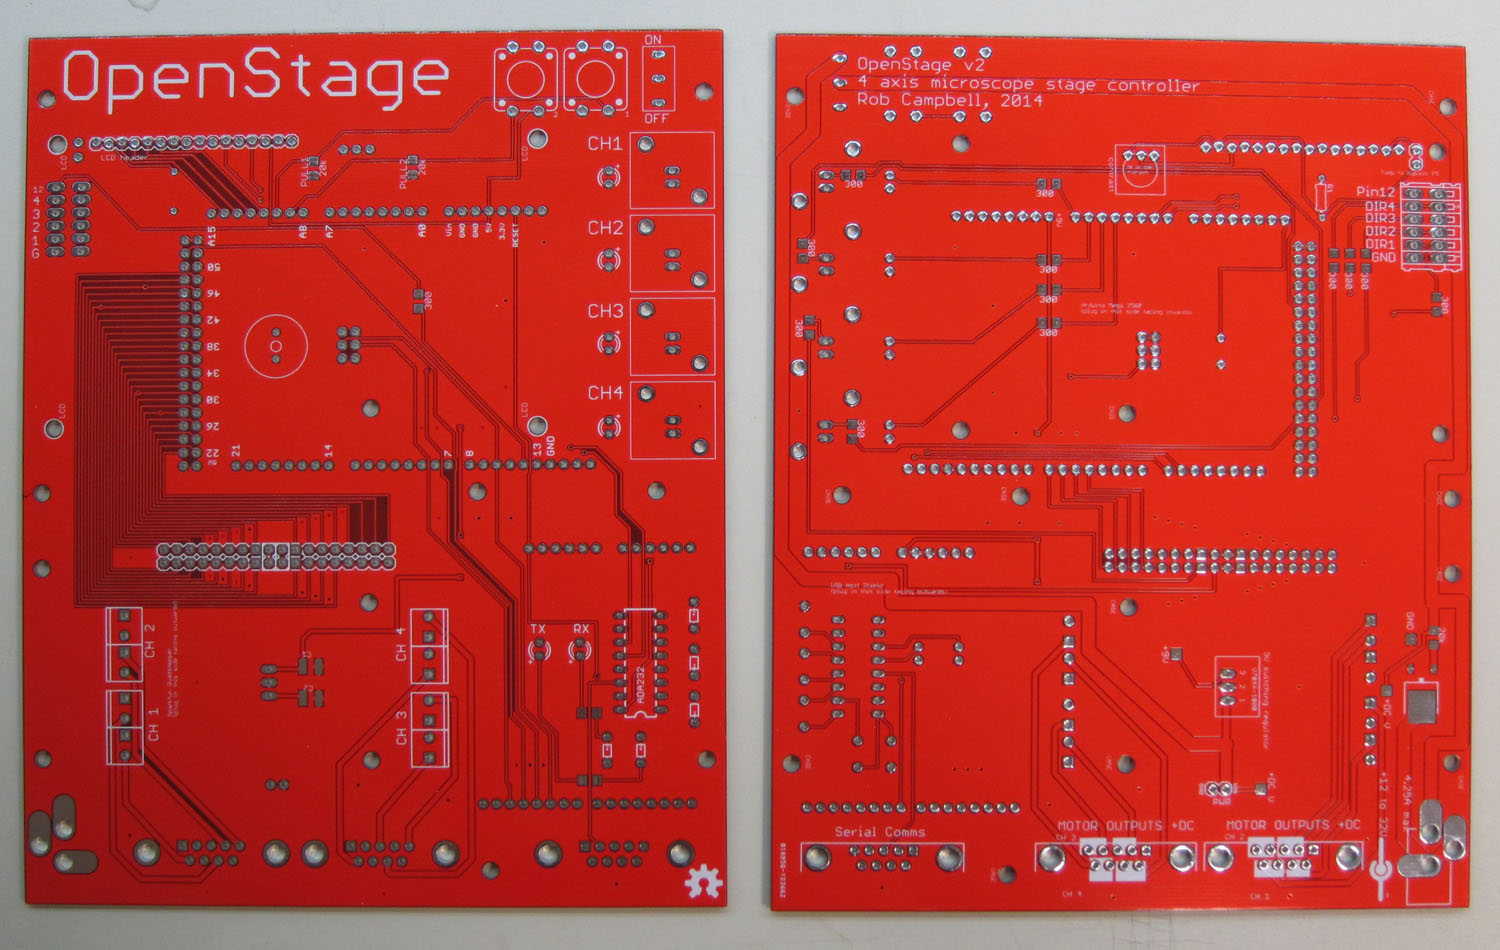
\includegraphics[width=5in]{IMG_3188.JPG}
\caption{Front (left) and back (right) views of the bare PCB.}
\label{frontback}
\end{figure}

\begin{figure}[!ht]
\centering
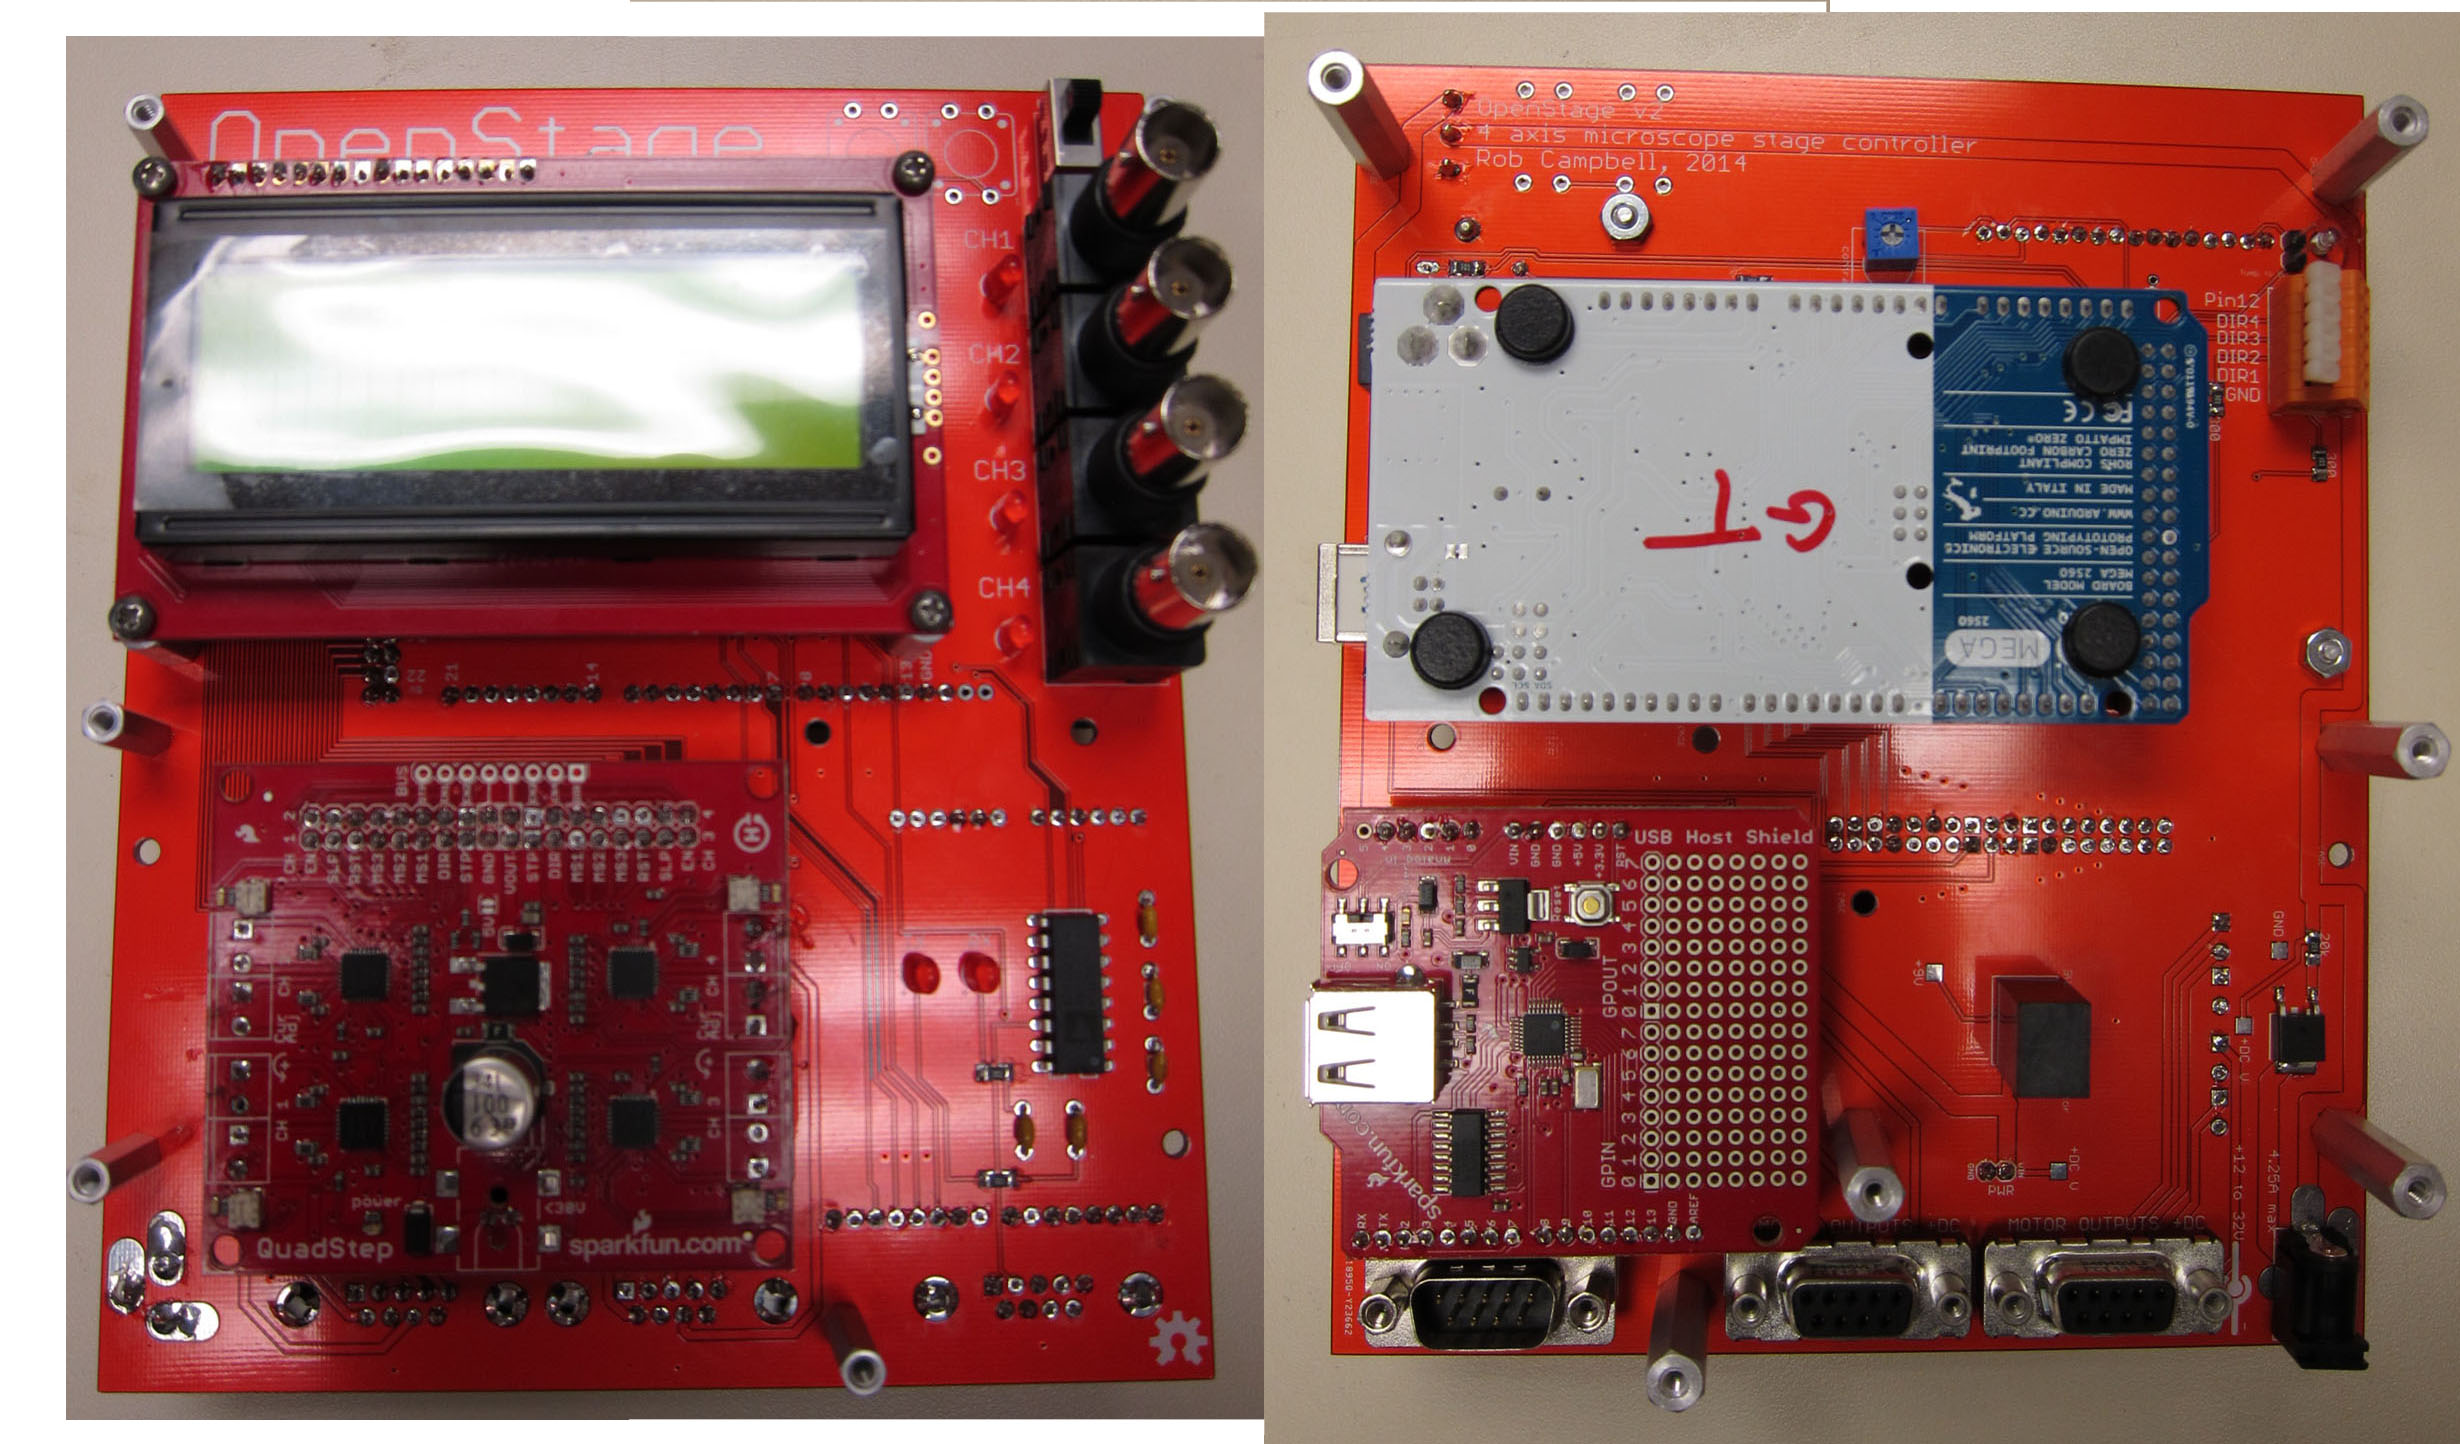
\includegraphics[width=5in]{finished_1.jpg}
\caption{Front (left) and back (right) views of the finished PCB.}
\label{finished_1}
\end{figure}

\clearpage

\section{Getting power to your board}
The first thing we'll do is hook up the components related to powering the board. You'll install the main power switch, input jack, the 9V regulator which powers the Arduino and USB host shield, and the MOSFET that is used for reverse current protection. 

Install the power switch (Fig.~\ref{switch}) so it's facing frontwards (i.e. the solder will be applied to the \textit{back} of the board). In Rev 2 boards the drill holes are too small for this switch and they've been expanded to allow the switch to fit. Solder will not take on the lower, unused, switch connection. This is not a problem. Next solder the power jack, MOSFET, and 20k resistor to the back of the board (Fig~\ref{switch}). The MOSFET and resistor are surface mount, so all the soldering is to the back face of the board. The power jack is through hole, so it's inserted into the back face and you solder to the front face. 



\begin{figure}[!ht]
\centering
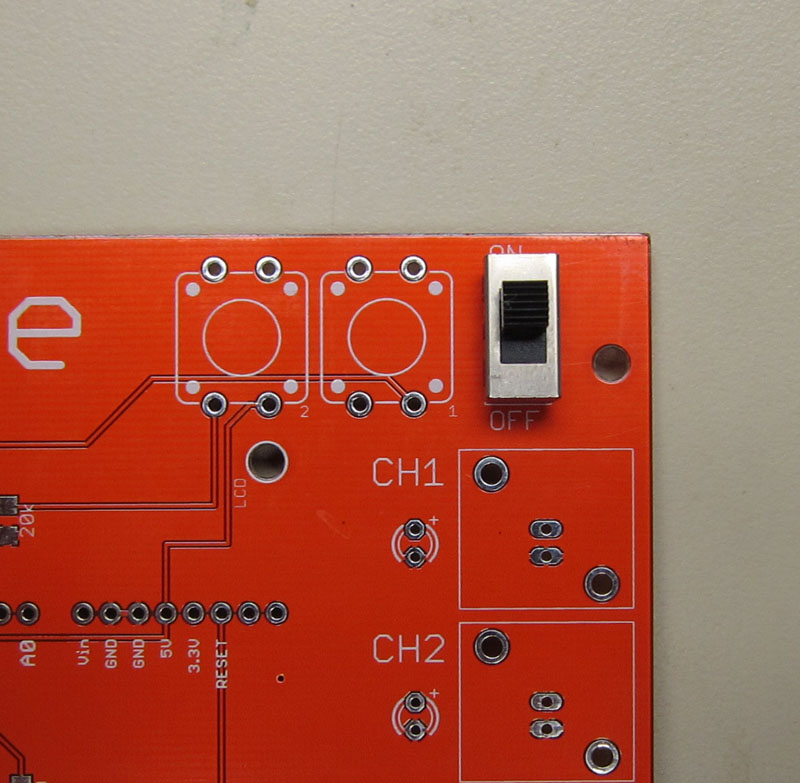
\includegraphics[width=3in]{IMG_3194.JPG}
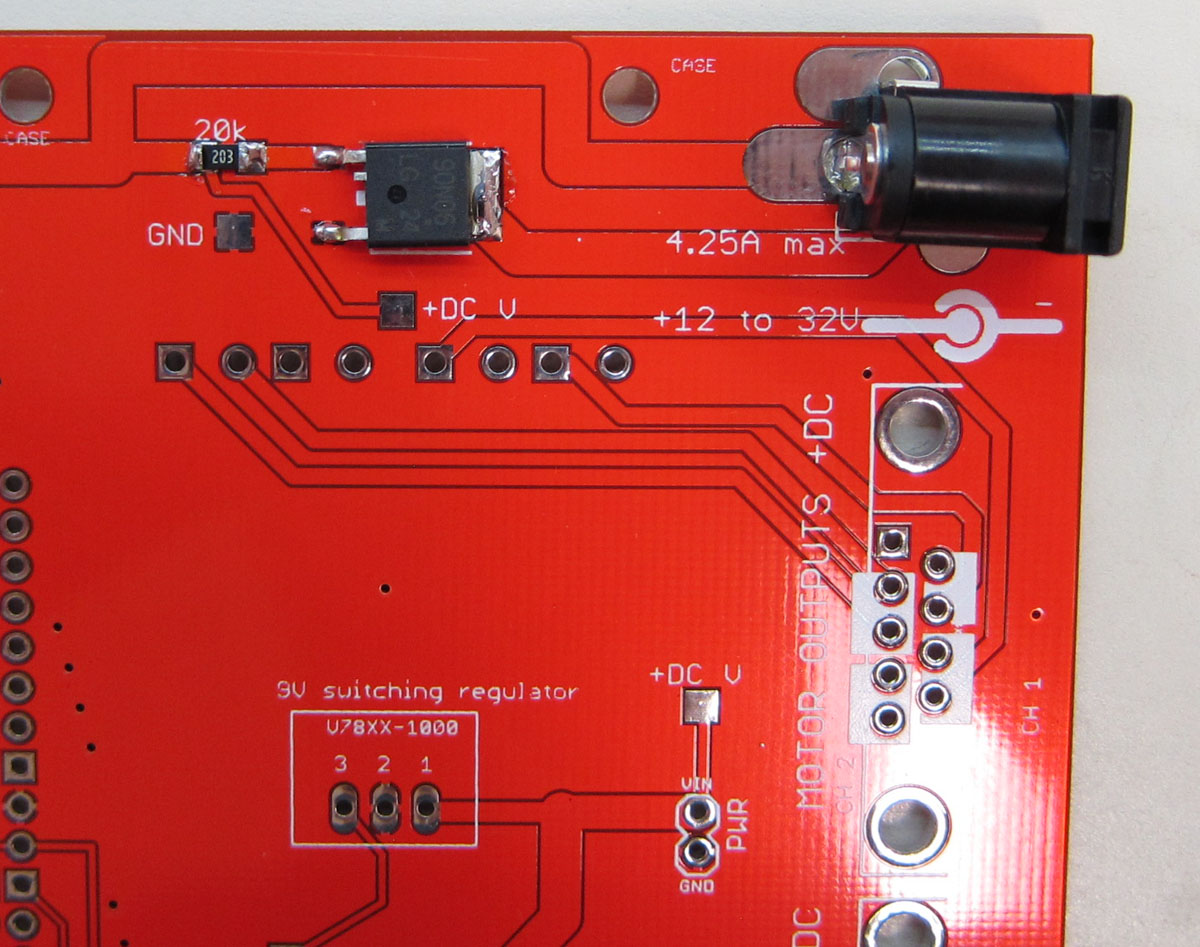
\includegraphics[width=3in]{IMG_3190.JPG}

\caption{Power switch (left). Power jack and reverse polarity protection (right).}
\label{switch}
\end{figure}

\clearpage

\section{Soldering small surface mount components}
Soldering the surface mount resistors is not too tricky once you have the technique down. First apply a little solder to one pad (Fig.~\ref{onePad}) then solder resitor to this pad with the aid of forceps (Fig.~\ref{forceps}). Finally, solder the remaining pad (not shown). 

\begin{figure}[!ht]
\centering
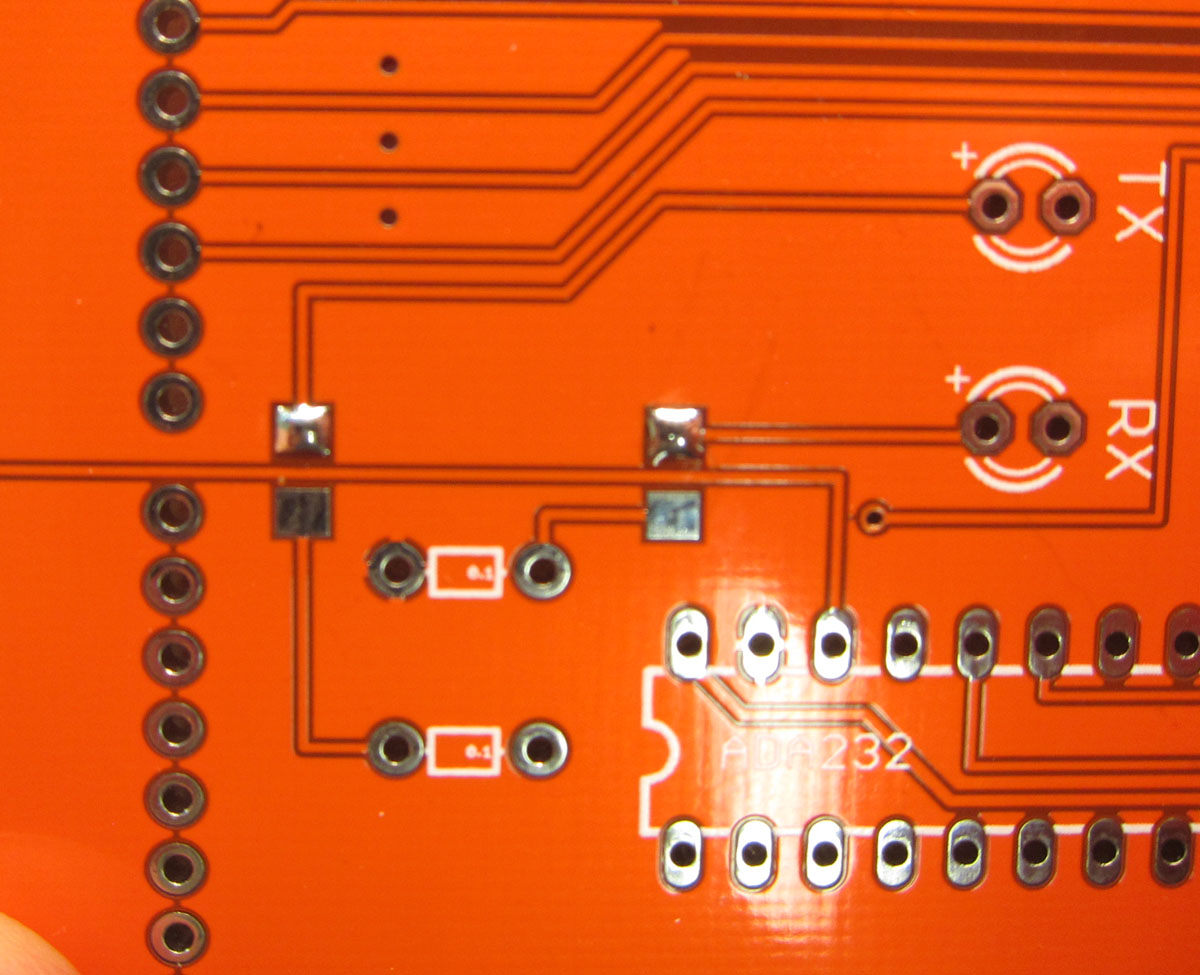
\includegraphics[width=4in]{IMG_3198.JPG}
\caption{Solder applied to one pad in preparation for soldering a resistor in place. Image shows two pairs of reistor pads. Solder has been applied to the upper pad of each pair. }
\label{onePad}
\end{figure}


\begin{figure}[!ht]
\centering
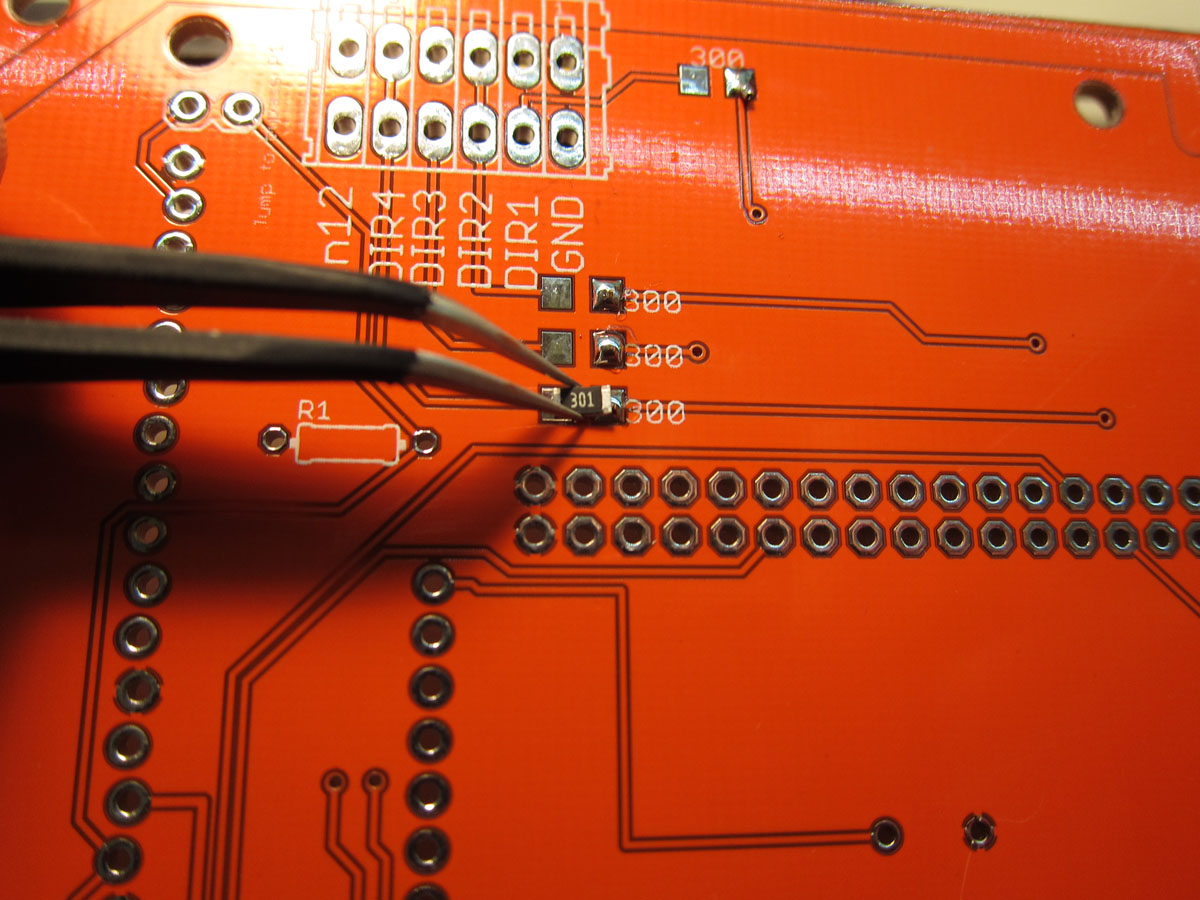
\includegraphics[width=4in]{IMG_3200.JPG}
\caption{Rest resistor on one pad. Keep in place with forceps. Apply solder.}
\label{forceps}
\end{figure}

\clearpage

Solder the two surface-mount capacitors to the front of the board (Fig.~\ref{9V}, left). The capacitor with the higher voltage rating goes on the input side of the regulator (the lower pair of pads, nearer the serial ports). Then solder into place the 9V regulator to the rear of the board (Fig.~\ref{9V}, left). The regulator has a dot indicating which pin is number 1. 


\begin{figure}[!ht]
\centering
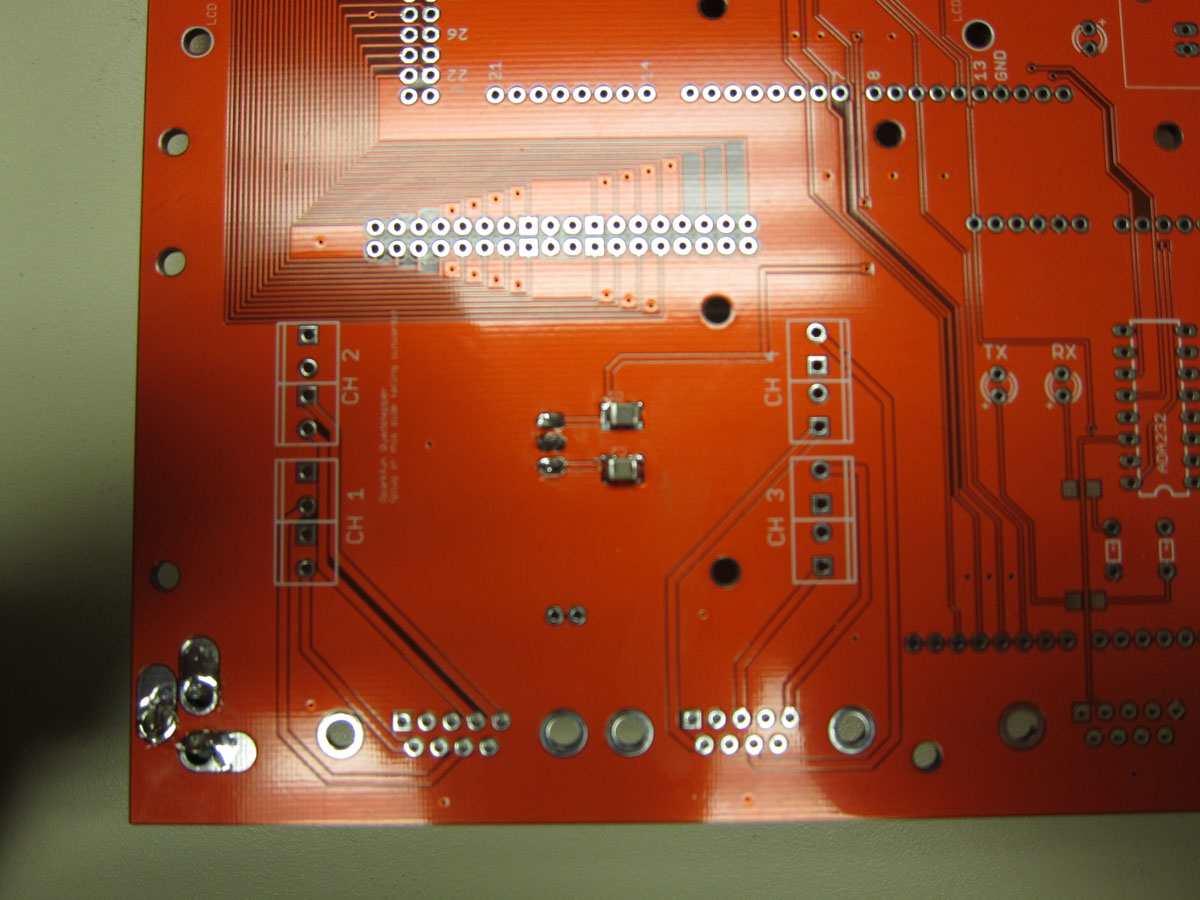
\includegraphics[width=2.3in]{IMG_3193.JPG}
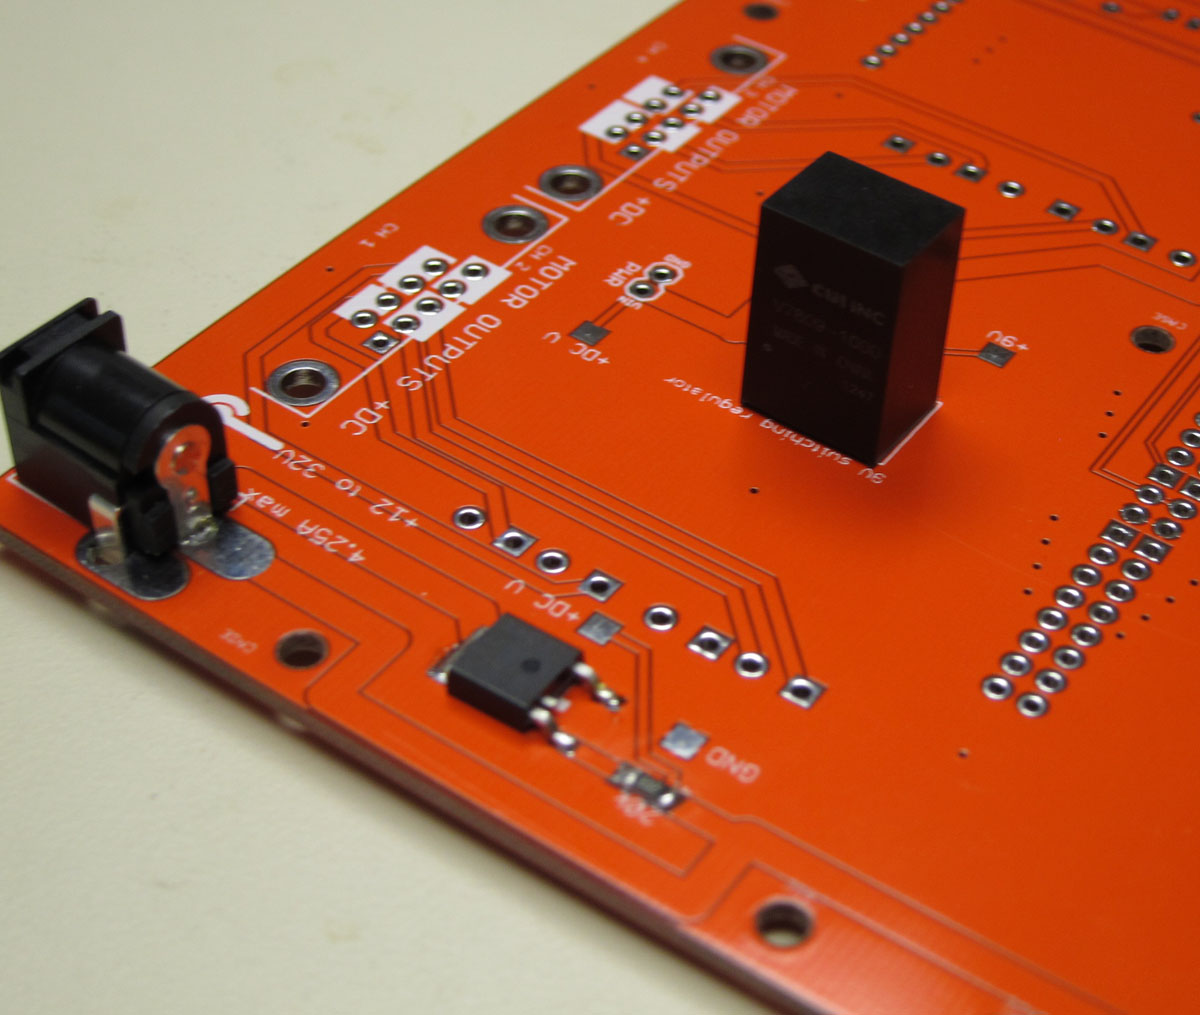
\includegraphics[width=2.3in]{IMG_3191.JPG}
\caption{Capacitors for 9V regulator (left). 9V regulator (right).}
\label{9V}
\end{figure}

\clearpage

\section{Testing the power}
At this point you have enough circuitry on-board to check that the power is being distributed correctly. Apply the probe leads across to points which ought to be supplying the full input voltage. The inputs to the QuadStepper are a good place (Fig.~\ref{power}, left). In the example images, we're using a 24V supply. We measure 24V when we do this. This should be under the control of the board's power switch. Next check that you get 9V after the regulator. You can use the 9V test pad and any ground connection (including the Quadstepper's ground you previously used to measure the full input voltage). This should read close to 9V (Fig.~\ref{power}, right). Finally, you can switch the polarity of the input jack if you wish. You should no longer be able to pick up a voltage. This indicates that the MOSFET-based reverse polarity protection is working as expected. 


\begin{figure}[!ht]
\centering
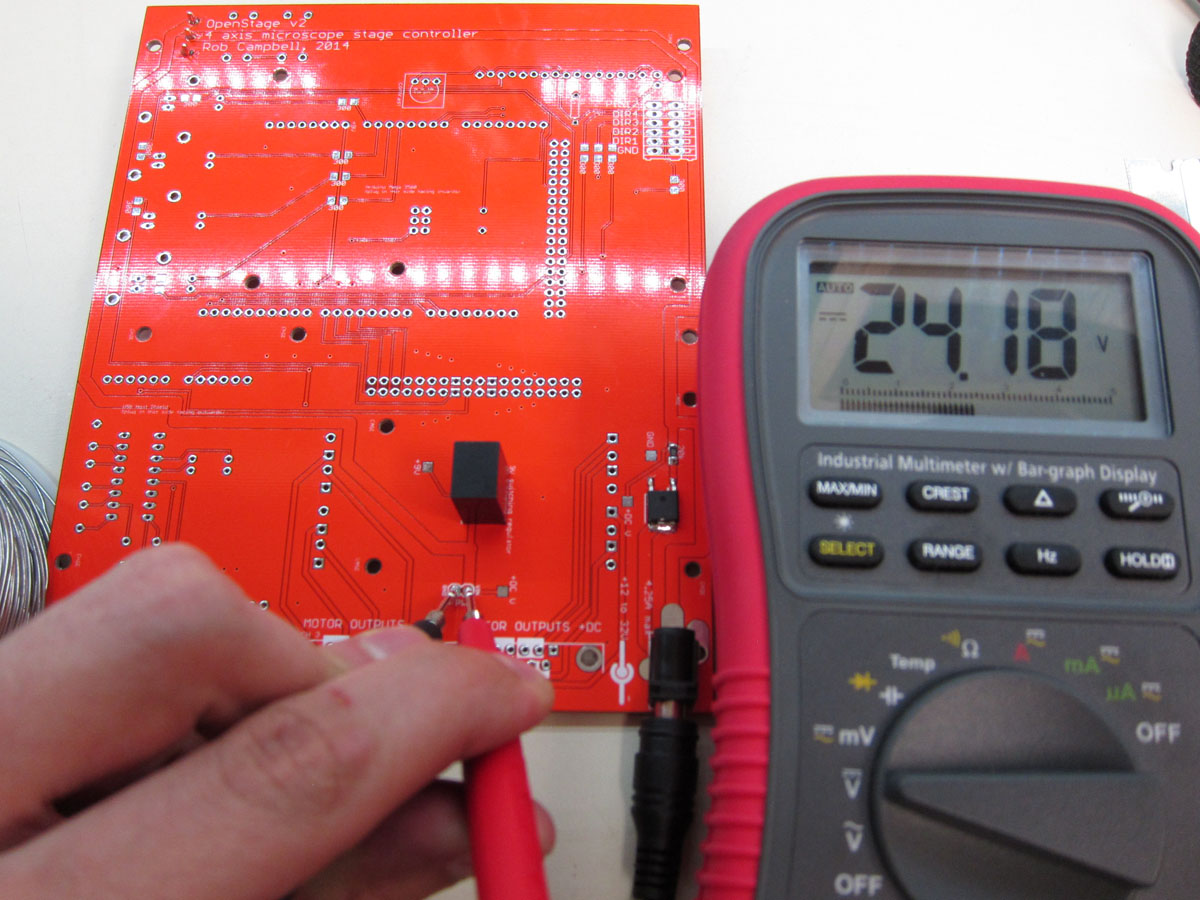
\includegraphics[width=2.5in]{IMG_3195.JPG}
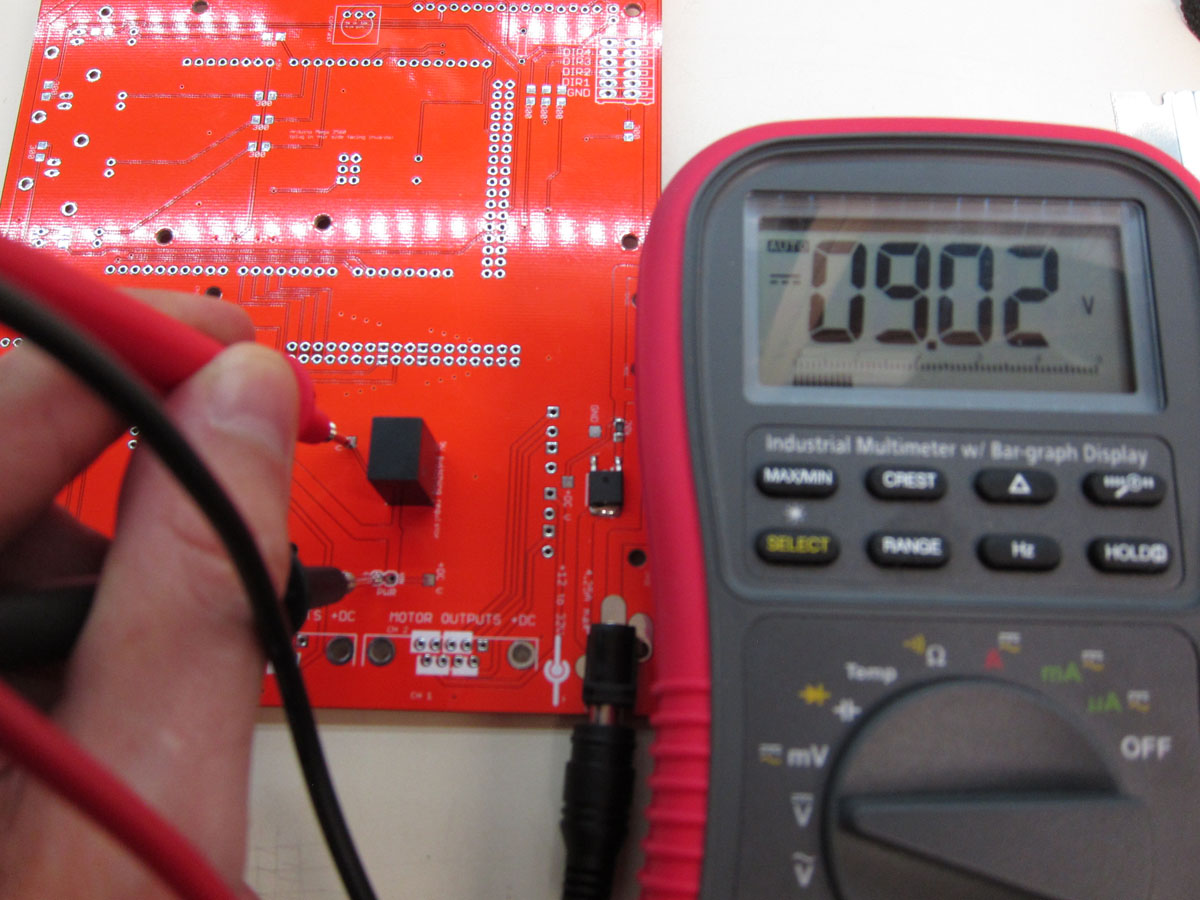
\includegraphics[width=2.5in]{IMG_3196.JPG}
\caption{Measuring input voltage (left), in this case 24V. Measuring output of 9V regulator (right).}
\label{power}
\end{figure}

\clearpage
\section{Attach small components}
Now is a good time to solder into place the smaller components. There are 15 resistors to attach. Six of these are current-limiting resistors for the indicator LEDs. If you want the LEDs bright then use a resistance of about 300$\Omega$. If you want them dim, then about 2500$\Omega$ to 3000$\Omega$ should do the trick. The remaining 9 resistors are current limiting resistors for the debugging lines; these are all 300$\Omega$. The buzzer is attached to the front face of the board. The ADM232 (Fig.~\ref{ADM232}) IC and associated capacitors attach to the front face of the board. Also shown in Fig.~\ref{ADM232} are the two indicator LEDs. These may have little `shoulders' on the pins that will prevent the LEDs from being fully inserted. If this is the case, you can clip away the shoulders. Insert the remaining 4 indicator LEDs. Attach the 5k$\Omega$ trim pot to the back of the board (Fig.~\ref{megaHeader}). Optionally, attach the Wago terminal connector for the debugging lines (Fig.~\ref{megaHeader}). 


\begin{figure}[!ht]
\centering
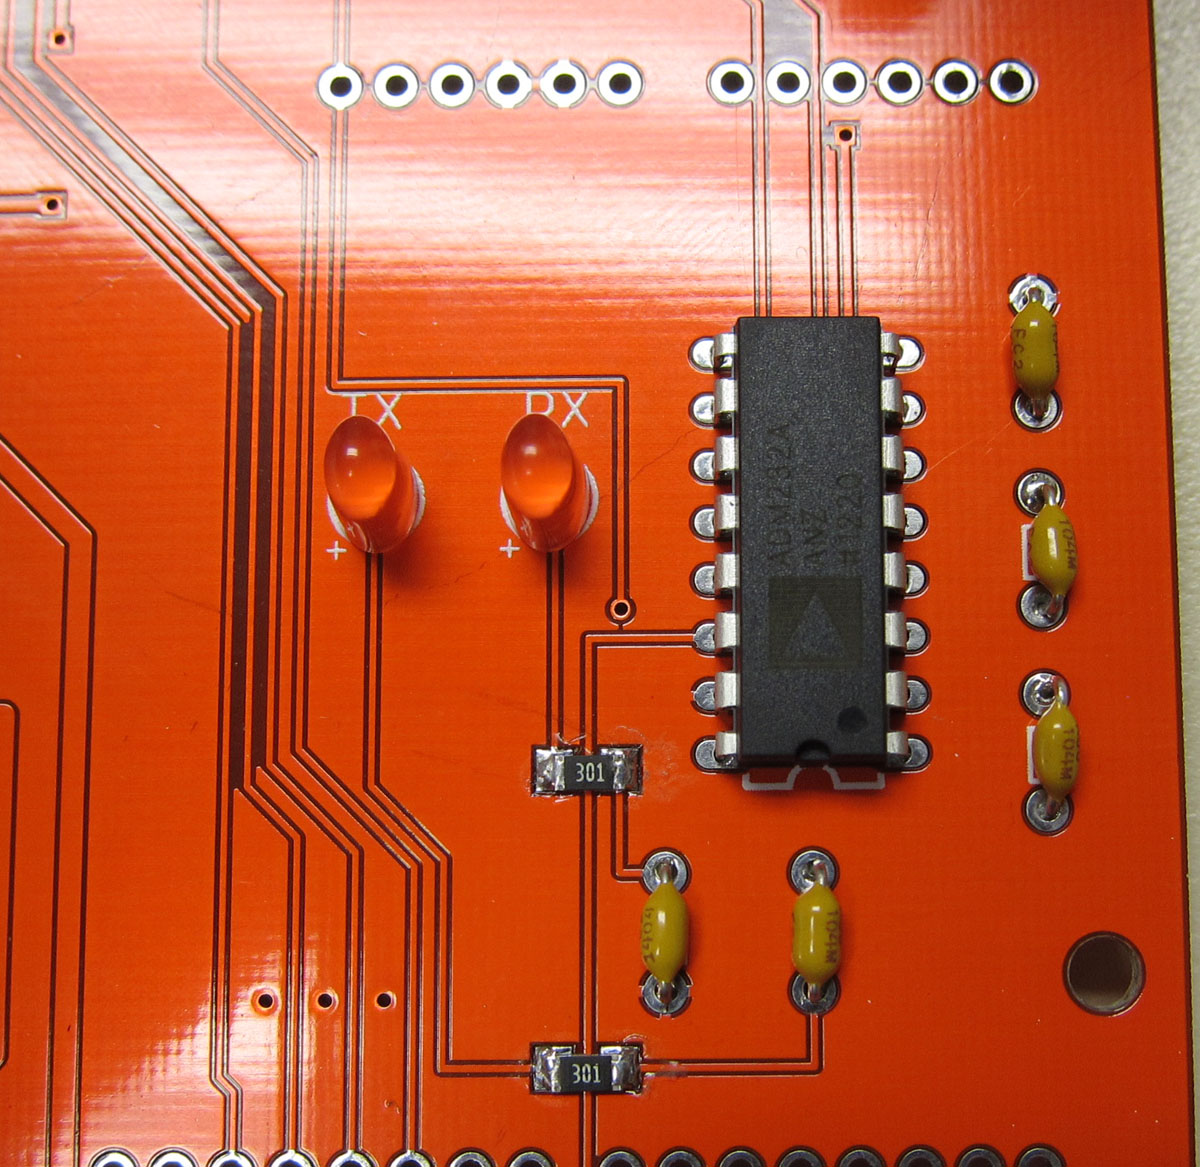
\includegraphics[width=4in]{IMG_3208.JPG}
\caption{ADM232 serial comms IC and associated capacitors.}
\label{ADM232}
\end{figure}

\clearpage

\section{Soldering the headers for the Arduino and USB host shield}
This is the most tedious bit but it's also the easiest to get wrong. Make sure the headers go into the correct side of the board. Let's start with the Arduino Mega male headers (Fig.~\ref{megaHeader}). These should be on the back face of the board. The idea is to have the Mega facing inwards on the back face, as shown in Fig.~\ref{megaHeader}. You will likely have to cut the single male rows from a longer strip. Once you're done here, do the headers for the USB host shield (Fig.~\ref{usbHost}). This also attaches to the back face of the OpenStage PCB. In this case we've soldered female headers to the OpenStage board and male headers to the USB host shield. It work equally well the other way around. 


\begin{figure}[!ht]
\centering
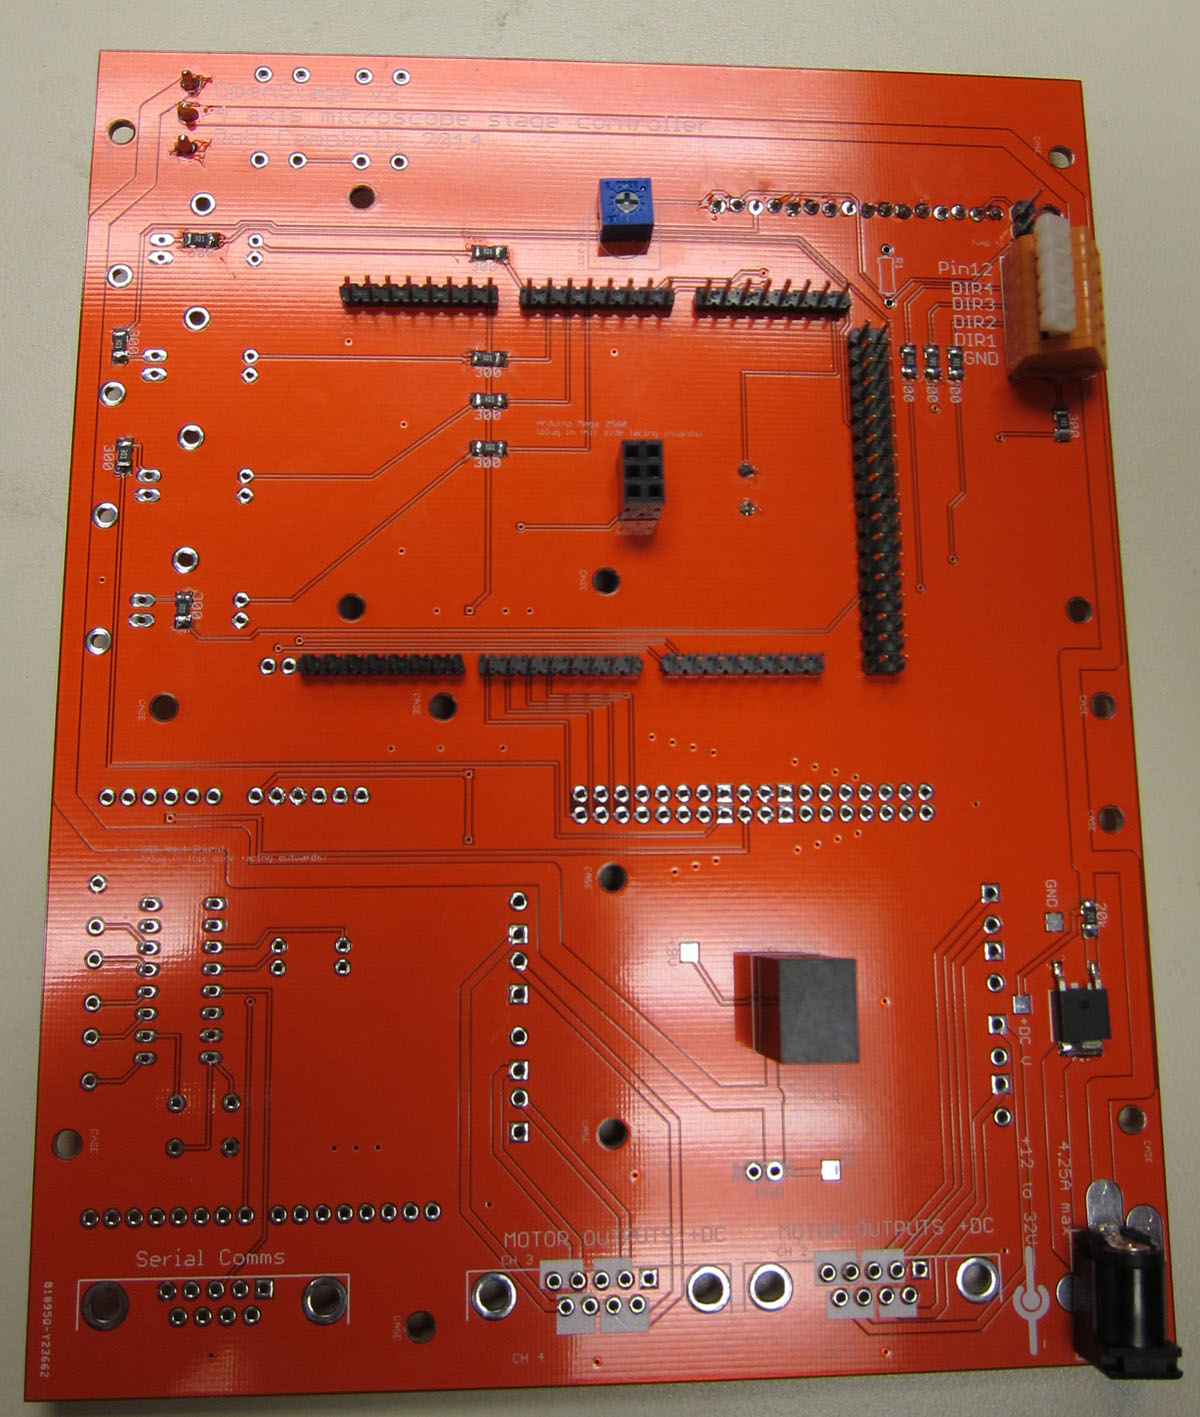
\includegraphics[width=4in]{IMG_3203.JPG}
\caption{Shows Arduino Mega headers, trim pot, and Wago terminal block. Note that the middle 2x3 header for the Mega is female.}
\label{megaHeader}
\end{figure}

\begin{figure}[!ht]
\centering
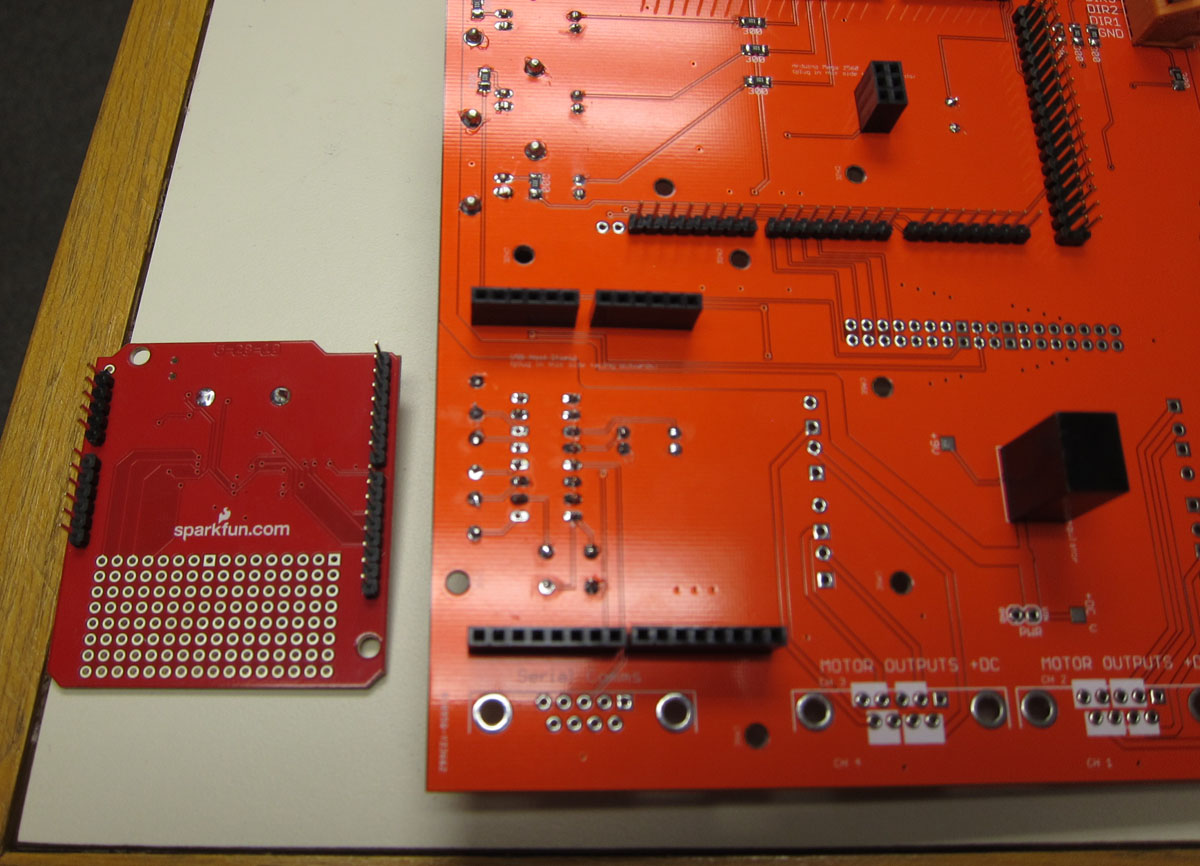
\includegraphics[width=4in]{IMG_3209.JPG}
\caption{USB host shield shown with headers attached. }
\label{usbHost}
\end{figure}

\clearpage

\section{Hooking up the Quadstepper}
Connecting the Quadstepper is a little more involved. First of all, you'll need to remove its power input jack. This is surface mount so you easily can snip off at the four attachment points. Then solder male headers to the underside of the newly-revealed 1x2 DC power connectors. Then attach male headers to the 2x19 strips. These are the digital control inputs for the motors. Again, these go on the \textit{underside} of the Quadstepper, so you can mount it facing outwards on the front of the OpenStage PCB (Fig.~\ref{finished_1}). Then solder the corresponding female adapters to the \textit{front} of the OpenStage PCB. 

The final step, the motor outputs, is a bit of an adventure. The pitch of these header holes is 0.15" and strip headers aren't available with this spacing. I've yet find a neat solution, so I present two options here. One, which allows you to easily remove the Quadstepper, is to attach male single pins to each motor output on the Quadstepper then cut 1x3 female adapters down to 1 pin and attach these to the OpenStage PCB. This looks like crap (Fig.~\ref{motoroutputs}, left), and you may need a glue gun get the female headers sitting properly before you solder them. Thus, an alternative is to solder the motor connections with short wires (Fig.~\ref{motoroutputs}, right). This looks nicer, but it means you can't get the Quadstepper off very easily. Given that there is no reason to remove it, the latter option might be the easier. Once you've done this, solder into place the two female DB9 sockets for the motor outputs. 


\begin{figure}[!ht]
\centering
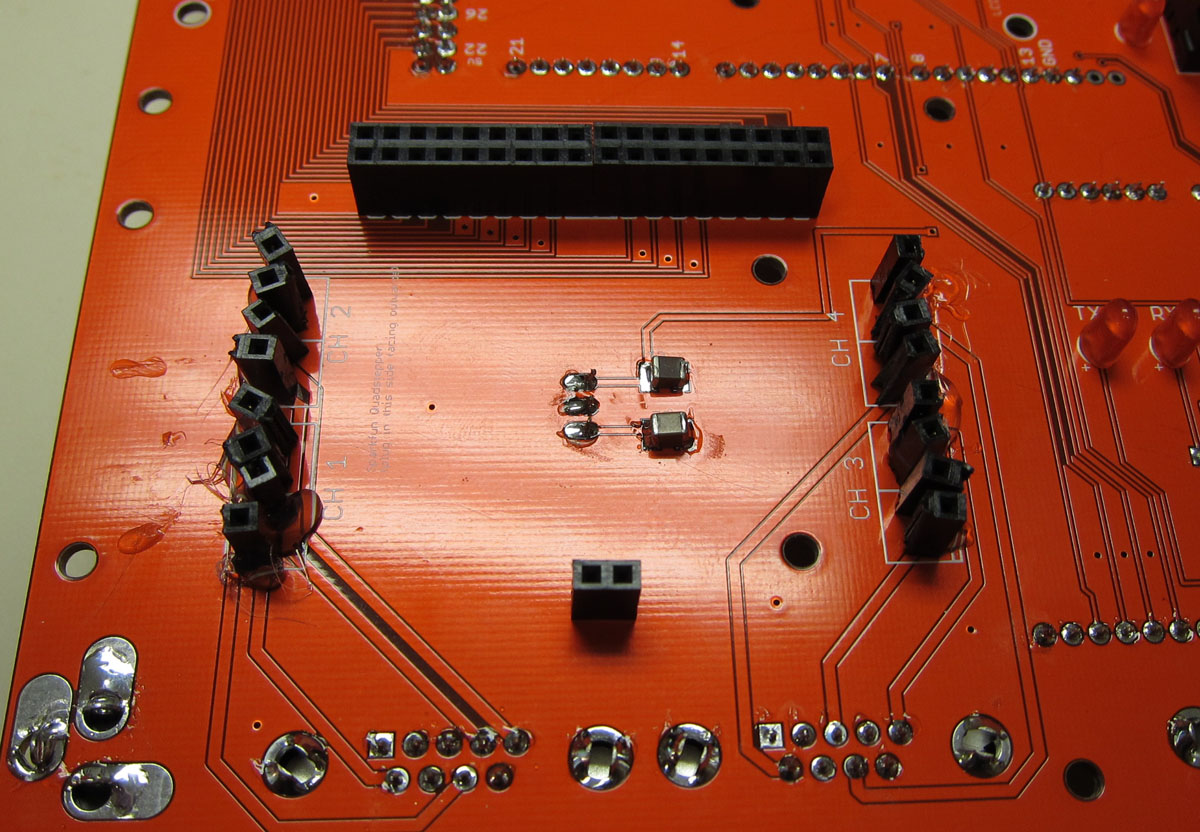
\includegraphics[width=3in]{IMG_3211.JPG}
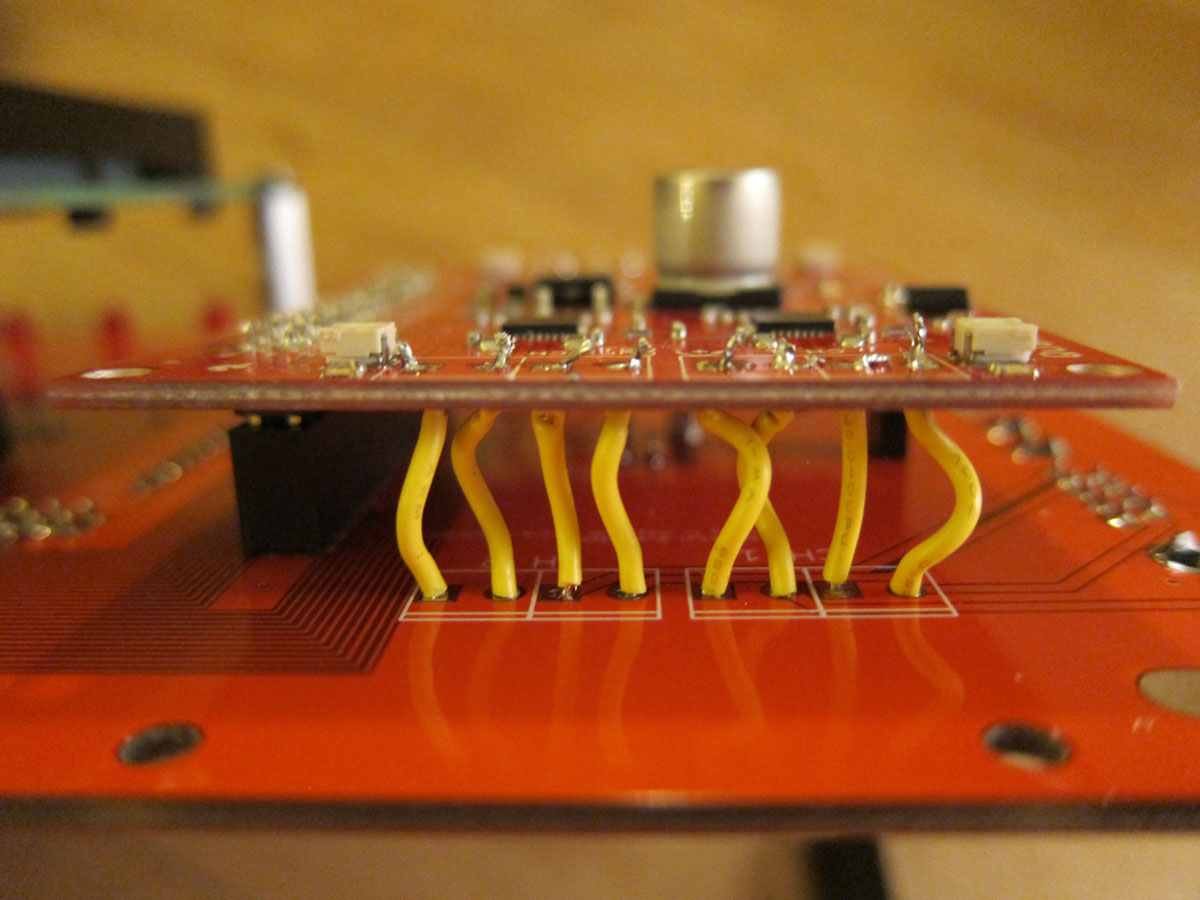
\includegraphics[width=3in]{IMG_3232.JPG}
\caption{Quadstepper female headers on OpenStage PCB (left) or using wires (right) }
\label{motoroutputs}
\end{figure}


\clearpage

\section{Wiring up the LCD display}
Because this a Rev 2 board, the LCD display won't just slot into place with a male and female header. This is because the connection on the board is inverted. To get around this, the easiest thing is to use a ribbon cable to invert inputs. You want to have something that looks like Figure~\ref{ribbon}. There are a bunch of ways you could do that. In the images shown, I've soldered a male strip header to the back of the LCD display. The 16 wire ribbon is soldered directly onto those pins. The other side of the cable has a female header on it. This female header connects to a 90 degree male header on the back of the OpenStage board. You could equally well solder directly the LCD. See how much space you have and what works best for you. If you wish to attach the BNC connectors next to the LEDs, you could do this now. These BNC connectors allow you to monitor the step pulse trains going to the motors.

\begin{figure}[!ht]
\centering
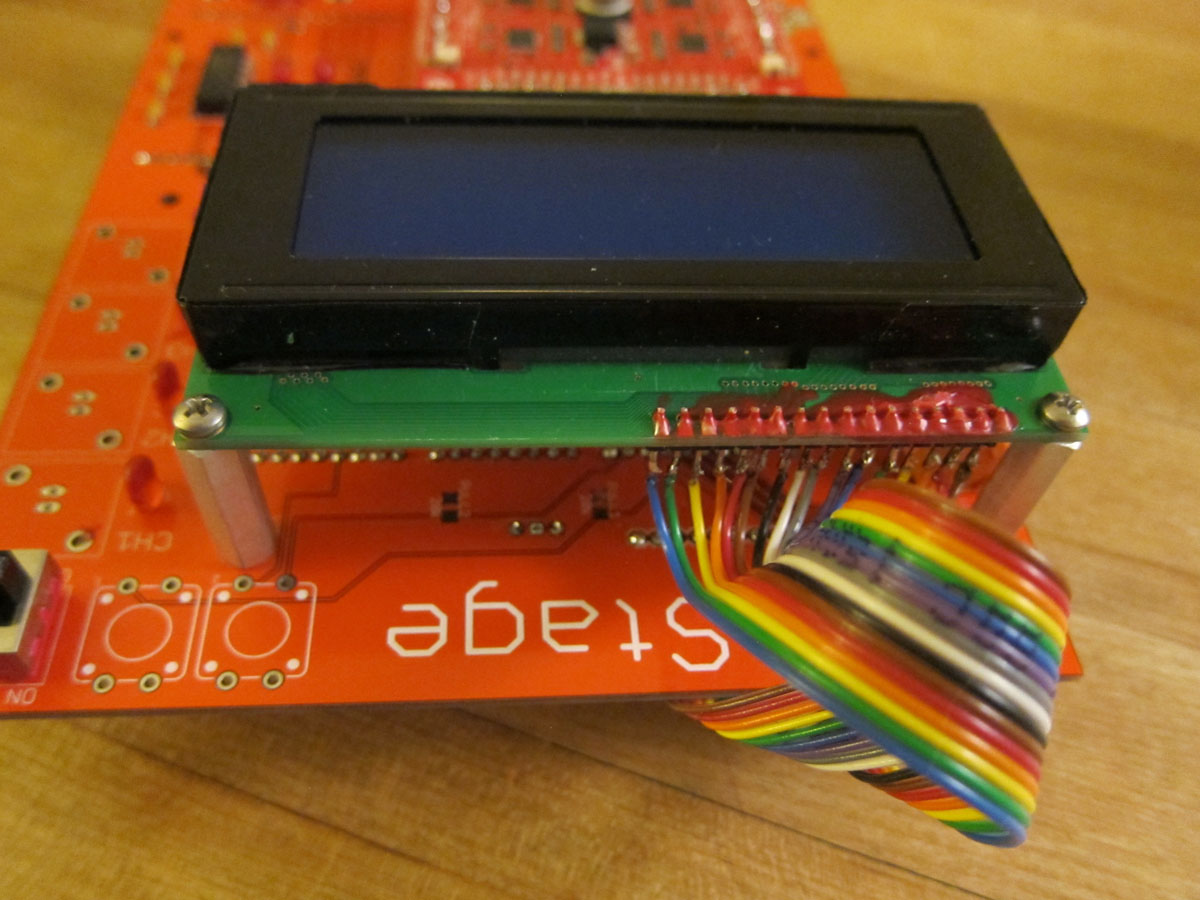
\includegraphics[width=3in]{IMG_3230.JPG}
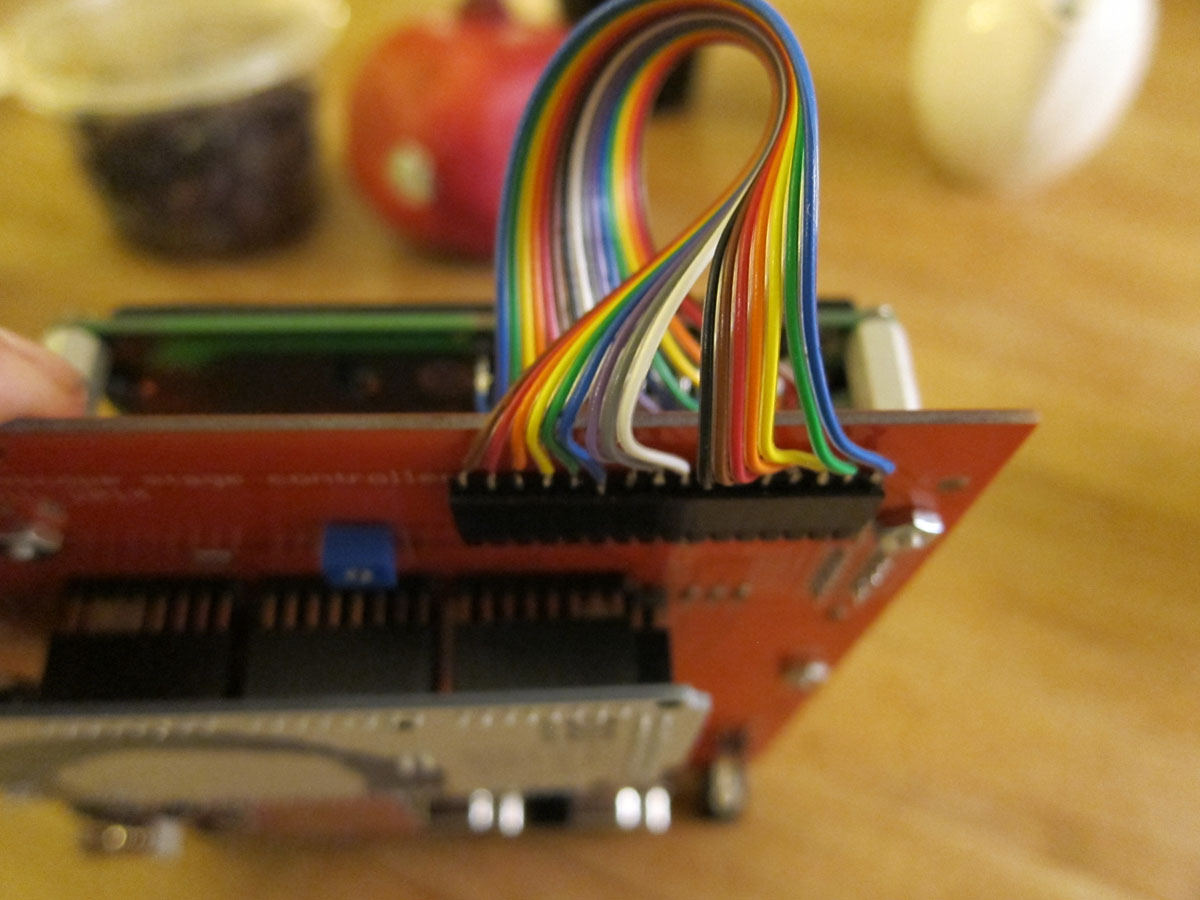
\includegraphics[width=3in]{IMG_3231.JPG}
\caption{Using a ribbon cable to invert the LCD inputs.}
\label{ribbon}
\end{figure}

\clearpage

\section{Connecting the motors to the DB9 cables}
Get a M/M DB9 cable and cut in half. Strip and expose the leads. You will be using 4 or 6 wire stepper motors. 6 wire steppers will have one pair of wires that aren't connected to anything. Stepper have two sets of coils inside and each set of coils is connected to one pair of wires. Use your datasheet or a continuity tester to figure out which wires form a pair. If you have 6 wire steppers, you will need the datasheet to make sure you avoid using the middle wires from each coil. Each row on the female DB9 connectors is for one motor. On the bottom row, pins 6\&7 connect to one coil and 8\&9 connect to the other coil. On the top row, pins 5\&4 form a pair and pins 3\&2 form a pair. Pin 1 is unused. It doesn't matter which coil connects to which pair of pins, but switching the coils will switch the default motor direction\footnote{There will soon be a way of switching default motor direction in the user settings section of the source code firmware. Currently, the only way is to switch the wiring.}.



\section{Uploading the firmware}
The board should now be assembled. Plug in the Arduino Mega, USB host shield, and Quadstepper. If it's not already programmed, hook up the Mega to a PC and upload the OpenStage firmare from the Github page (\textit{https://github.com/raacampbell13/openstage}). You can download as a zip (easy) or clone the repository (if that's your thing). 

If you haven't programmed an Arduino before, here's what you'll need to do. Download the Arduino IDE from \textit{arduino.cc}. Install the IDE. The source code for the OpenStage firmware is in the `\textit{OpenStage}' sub-directory from the Github repository. There are a bunch of source code files here. Unless you want to make significant changes to the firmware, you don't need to be concerned with most of this. All you care about is the user settings file. There are a bunch of different potential user settings files, depending on the desired configuration of the stage. We want the c\_userSettings\_MEGA\_PCB file. This file should have the extension `.ino'; if it has `.BAK', or any other extension, then rename the file. It should be called `\textit{'c\_userSettings\_MEGA\_PCB.ino'}. When you try to compile the firmware, the Arduino IDE simply concatenates the .ino files in the directory then compiles the resulting, larger, file. You don't want it to include any of the other c\_userSettings* files. So either delete them or make sure none of them end in .ino 

Now you're good to go! Open the file `\textit{OpenStage.ino}' in the Arduino IDE. When you do this, a new window will pop up and it will have about a dozen tabs. Each is a source file (.ino file) from the directory. Go to the tab called c\_userSettings\_MEGA\_PCB. If that tab doesn't exist, you didn't rename the file correctly. If there are any other tabs starting with `c\_' then you didn't remove or rename the extra settings files. If you have such issues, close the IDE and rename files to fix the problem. In the c\_userSettings\_MEGA\_PCB tab you can modify the user settings for your rig. You will want the LCD display and, presumably, the game pad, so don't alter the first three lines. If you want to communicate with the stage via the Arduino USB port, not a regular serial port, then change the value of controlViaUSB to 1. 

You will need to carefully set the `Microscope axis hardware definitions.' If you want three axes then leave the first bit of that section (up to `gear ratio') as is. What you likely will need to do is modify the gearRatio vector. Those numbers indicate the number of microns the stage will advance when the micrometer rotates revolution. e.g. The standard ThorLabs micrometers are 100 turns per inch; the imperial units advance 635 $\mu m$ per revolution and the metric ones 500 $\mu m$ per revolution. Each axis can have a different value, allowing finer motions for $z$, say. Similarly, you will need to define the number of degrees the stepper motors advance when they take a full step. Chances are you will have motors which are 1.8 degree (200 steps per revolution) or 0.9 degree (400 steps per revolution). Armed with these two pieces of information, OpenStage can determine its relative position in space with very high accuracy. 

The remaining parameters are less critical. They relate to things such as the speeds and step sizes that the PS3 game pad produces and the default speeds on each axis for PC-based control. Many of these settings can be altered via the serial port. You won't need to change the pin definitions at the end of the file. 

\section{Powering up!}
You're now ready to power up. Connect your power line and PS3 game pad. Hook up the motors (do not plug or unplug the motors with the power on). If you want computer control, hook up the USB cord or the serial port to your PC. To begin with, it might be sensible not to connect the motors to the rig. Attach little pieces of tape to the spindle to watch them move. Make sure the switch on USB host shield is set to `on'. Switch on OpenStage. You should see a `Booting...' message on the LCD display. The boot sequence should complete in about 5 seconds. Once it has booted you can control the stage using either a PC or the gamepad. 

The Quadstepper has 4 potentiometers, one for each motor. These control how much current is delivered to the coils. The power supply determines the voltage to the coils. If the current is too high the motors and the driver chips can run \textbf{very hot}. It shouldn't be necessary to run at high currents. Choose a low current at work your way up. You shouldn't need a heatsink on the motor. You might like to add a heatsink to the driver chips; again, however, this likely isn't necessary as they should be running cool. If the current is too low the motors will skip (see below).


\subsection{Control via gamepad}
The PS3 gamepad serves as a comfortable input device. The LCD displays current speed and position of each axis. The display is updated regularly, except at the fastest speed mode (see below) where it updates only at the conclusion of motion. 
The PS3 DualShock controller provides the following functionality:

\begin{itemize}
\item \textit{Analog control} of speed and direction for each axis is
  provided by the two analog sticks. The left stick controls X and Y and the right stick controls Z, and the 4th axis (z) if this is enabled. Larger stick displacements are mapped to higher motion speeds, making it easy to manually guide the stage at exactly the desired speed.
\item \textit{Fixed-size motion steps} are provided by the direction
  pad (D-pad). For instance,
  pressing the left D-pad button moves the stage one increment to the
  left. By default the D-pad controls X/Y motions; holding down the
  Triangle button whilst pressing up or down on the D-pad yields fixed
  step size motions in Z, with Triangle plus L/R yielding motions in z. 
\item The two shoulder buttons (L1 and R1) allow the user to cycle between 4
  different \textit{Speed Modes}. The selected speed mode influences
  both the maximum speed of analog stick motions and the size of the
  D-pad motion steps. Speed mode \#1 provides a nominal maximum speed
  of $3~\mu m/s$, \#2 is $25~\mu m/s$, \#3 is $100~\mu m/s$, and \#4 is
  $750~\mu m/s$. The size of the D-pad steps range from $3~\mu m$ to
  $50~\mu m$. Changing the speeds and motion steps sizes involves only
  trivial modifications to the source code (see above). The currently selected
  Speed Mode is indicated by the 4 LEDs on the DualShock. The stage boots in a low speed mode for safety reasons. 
\item The user can \textit{store} up to 4 locations and return to them
  later using the 4 right-hand buttons. Firmly press on a button for 1 second to store the current stage position. The controller produces an audible
  indication when a new location is stored. Return at any
  time to the stored location by double-clicking on the corresponding
  button. OpenStage returns to the stored position at maximum speed, as defined in the settings file. 
\end{itemize}


\subsection{Control via PC}
The Github repository contains a directory called `\textit{serialInterfaceScripts}.' Within this directory are sub-directories containing scripts for controlling the stage via MATLAB, Python, or LabView. The MATLAB functions are the most mature and well tested. The Python and LabView stuff has been verified to work but so far not used beyond this. 

To get the MATLAB scripts working, add the directory which contains the files to your MATLAB path. Edit the \textit{connectOpenStage.m} file so that it points to the correct serial port. Save the file. The first time you run one of the commands in that directory it will automatically try to connect to the stage. Try running OS\_getInfo, which queries the stage for a bunch of useful information. You should see MATLAB attempt to form a connection with the stage then a bunch of information will appear on the screen. If this occurs, then you have a connection back and forth with the stage. If it doesn't, find out why. 

The rest of the functions should be fairly self-explanatory. OS\_getPosition returns the current position of each axis in microns. OS\_goto will move the stage, by default motions are to an absolute position but it also does relative positions. See its help docs. OS\_beep works the speaker. OS\_zero will zero the LCD counters. Calling some functions, such as OS\_stepSize with no input arguments will cause the stage to report the current step size. Add the appropriate input argument and a new step size is set. \textbf{NOTE: do not use full steps! See below for why.}

\subsection{Accuracy}
The stage should have relative accuracy of well under a micron. i.e. you should be able to make many motions in different directions then return to zero and be in virtually the same position give or take half a micron or so. If this isn't happening then likely you have an issue with the motors skipping. It would be wise to take the time to read our paper, as it describes in detail the steps you can take to get high accuracy motions. The information in the paper is summarized below. 

The stage controller has no feedback. It issues motion commands as TTL step pulses and the motors make small steps of a known size each time a pulse is received. If the motors fail to step, the OpenStage controller won't know and you'll get under-shoots. Under normal use conditions, the motors are \textit{very reliable} and skipped steps are not an issue. We have run our system for months and had no problem with this. The motors will step virtually 100\% of the time when told to do so. If they are failing to step then something is wrong. The main cause of skipped steps is lack of torque: you're asking the motors to move a load they cannot push. If this happens they'll skip steps and usually this skipping is very obvious (often a grating noise occurs). 

In a stepper motor, torque decreases with increasing speed. So moving too fast will cause skipped steps. The higher the load on the motors, the lower the maximum speed. If you accelerate too quickly the motors may skip. If the current is too low, the motors will skip. If you're using full steps, it's very likely you will get many skipped steps unless the motor current is set \textit{just right}. So avoid full steps. Half steps and smaller are much smoother and won't skip. If you don't know anything about stepper motor microstepping, then do a little Googling or read our paper.



\end{document}





 
